\documentclass[a4paper, 12pt]{book}

\usepackage[T1]{fontenc}
\usepackage[utf8]{inputenc}
\usepackage[italian]{babel}
\usepackage{graphicx}
\usepackage{sidecap}
\usepackage{subfig}
\usepackage[colorlinks]{hyperref}
\hypersetup{linktoc=all}
\newcommand{\foto}[1]{\includegraphics[width=0.5\textwidth]{#1}}
\usepackage{listings}



\begin{document}
    
\author{Giovanni Tosini}
\title{Sistemi Operativi \\
\large Secondo semestre}
\date{ }
\maketitle
\newpage
\tableofcontents
\newpage

\chapter{Monitor}

Si tratta di una struttura simile ai semafori, implementa di default la mutua esclusione. Simile a una classe di un linguaggio a oggetti, può contenere:
\begin{itemize}
    \item variabili(sono private)
    \item metodi(solo loro possono utilizzare le variabili definite all'interno del Monitor)
    \item costruttore
\end{itemize}

Quando un processo usa una entry del Monitor, gli altri non possono accedervi. Al suo interno posso dichiarare variabili di tipo CONDITION, non hanno valore, vengo usate esclusivamente con i metodi WAIT e SIGNAL.

\begin{verbatim}
    CONDITION x
    x.wait -> blocca il processo, non avvengono incrementi
              o decrementi come con i semafori
    x.signal -> se fatto quando non ci sono processi in
                attesa, non fa niente
\end{verbatim}

\begin{center}
    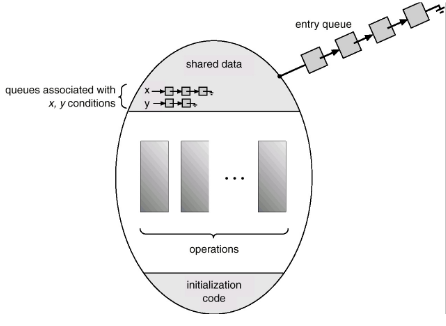
\includegraphics[width=0.5\textwidth]{ovetto.png}
\end{center}

Il comando SIGNAL può rompere la mutua esclusione, perché un eventuale processo fermo potrebbe ripartire e in quel caso entrambi sarebbe all'interno della sezione critica, per evitare ciò il processo che la chiama:
\begin{itemize}
    \item viene bloccato
    \item oppure SIGNAL deve essere l'ultima istruzione prima di uscire dal Monitor
\end{itemize}

Quale metodo usare? Dipende dal Monitor.

\section{Problematiche}

\begin{itemize}
    \item esistono pochi linguaggi che li implementano
    \item possono essere applicati solo quando ci sono processi che condividono la memoria(stessa macchina)
\end{itemize}

\chapter{Deadlock}

Causato quando un processo è in attesa di un evento causato a sua volta da un altro processo in attesa.
Ci sono quattro condizioni che possono causare un Deadlock:

\begin{itemize}
    \item mutua esclusione
    \item hold and wait: processo che detiene una risorsa ed è in attesa di una risorsa utilizzata da un altro
    \item no preemption: il processo deve rilasciare volontariamente la risorsa(non può essere ucciso)
    \item catena circolare: A attende B, che attende C, che attende A
\end{itemize}
In presenza di tutte e quattro esiste la possibilità che si verifichi.
Tecnica di prevenzione: basta che una delle quattro non venga rispettata e il Deadlock non può avvenire.

\paragraph{Modello astratto RAG (Resource Allocation Graph)}

\begin{center}
    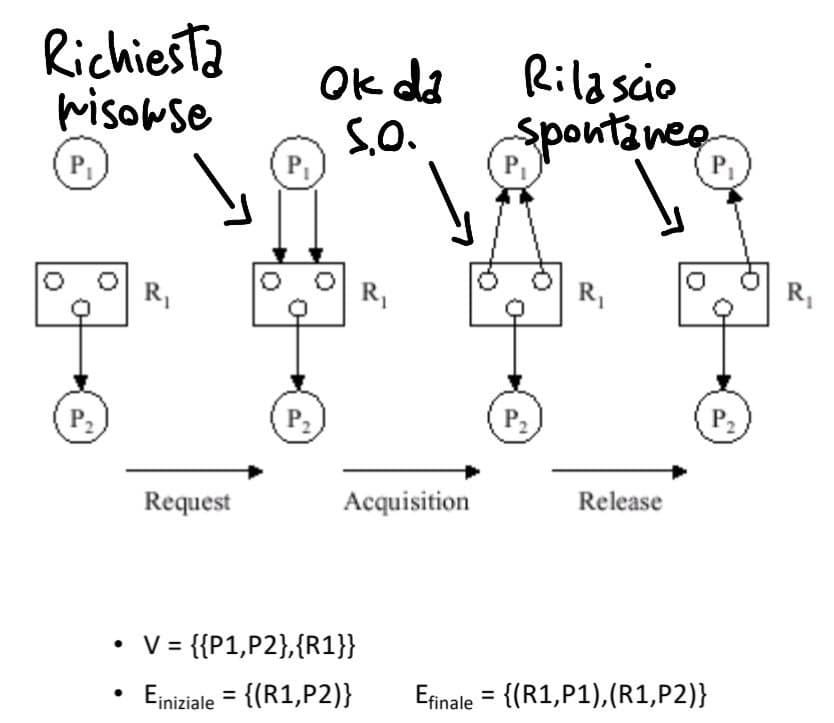
\includegraphics[width=0.5\textwidth]{rag.jpg}    
\end{center}
In generale, se abbiamo una sola istanza di ogni risorsa e siamo in presenza di un ciclo, il Deadlock è certo.
Con risorse con più istanze invece non è assicurato.

\section{Gestione Deadlock}

Prevenzione statica: evitare ovvero che si verifichino una della quattro condizioni sopra riportate,
se ci sono risorse disponibili non le assegno a prescindere.

\begin{itemize}
    \item mutua esclusione: non posso toglierla
    \item hold and wait: accumulo tutte le risorse tutte in una volta altrimenti non procedo
    questo porta a delle problematiche:
    \begin{itemize}
        \item basso uso delle risorse
        \item starvation
        \item occorre conoscere le risorse necessarie
    \end{itemize}
    \item no preemption: un processo che richiede una risorsa non disponibile
    sarà costretto a rilasciare tutte le altre risorse che stava tenendo
    \item ogni risorsa avrà una priorità crescente, il processo può richiederle esclusivamente in ordine crescente
\end{itemize}
Prevenzione dinamica, durante l'esecuzione si blocca un processo in base al RAG, occorre conoscere  a priori il caso peggiore 
in cui si causa un Deadlock e permette di sfruttare maggiormente le risorse per altri processi diversamente da quella statica.
Guardando il RAG, come un processo richiede una risorsa ipotizza di concederla e verifica se si presenta un ciclo,
in caso affermativo la richiesta verrà rifiutata, il processo rimarrà in attesa e il sistema resterà in 
un stato SAFE.

\vspace{3ex}
\begin{tabular}{|c|c|c|}
    \hline
    x & Richieste & Possedute \\
    \hline
    p0 & 10 & 5 \\
    \hline
    p1 & 4 & 2 \\
    \hline
    p2 & 9 & 2 \\
    \hline    
\end{tabular}

\vspace{3ex}p0 avrà bisogno di 10 istanze delle quali già ne possiede 5,12 sono quelle presenti, 9 in uso e 3 libere.
Stato SAFE o UNSAFE? Si va in ordine per processo:

\begin{itemize}
    \item p0 ne sta usando 5, ne occorrono altre 5, con le 3 libere non può essere soddisfatto, di conseguenza rimarrà in attesa
    \item p1 ne chiede 4, ne ha già 2, 3 sono libere, di conseguenza se andasse prima lui ne avremmo 5 libere dopo
\end{itemize}
Quindi saremmo in uno stato SAFE.\\
N.B.: lo scheduler in tutto ciò non ha rilevanza, lui si limita a scegliere quali processi mettere nella CPU.

Lo svantaggio della
previsione dinamica è l'uso delle risorse minore, perché ci possono esserne alcune che non vengono sfruttate.

\vspace{3ex}1) L'algoritmo RAG funziona solo con risorse che possiedono un'unica istanza, funzionamento:

\begin{itemize}
    \item aggiungo al RAG l'arco di reclamo, ovvero in futuro quel processo richiederà l'uso di quella risorsa molto probabilmente
    \item il S.O. permetterà al processo di usare la risorsa solo se ipotizzando che venga fatto, non si verifichi un ciclo
\end{itemize}

\begin{center}
    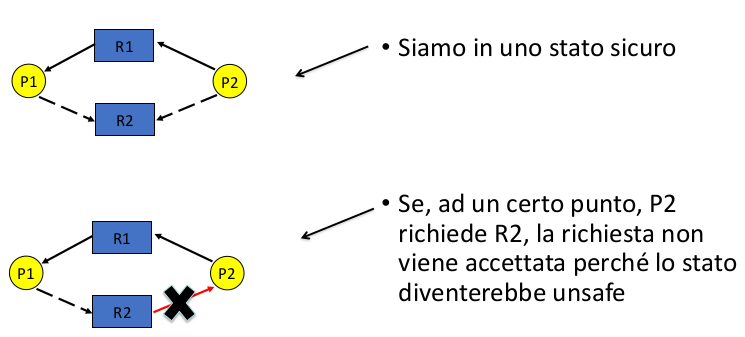
\includegraphics[width=0.8\textwidth]{rag_reclamo.png}
\end{center}
La freccia tratteggiata indica l'arco di reclamo.

2) L'algoritmo del banchiere è meno efficiente dell'algorimo RAG, ma
funziona con qualsiasi numero di istanze delle risorse. Si divide in due parti, una che simula la cessione dell'istanza della risorsa
e una che ne verifica l'effetto.

\begin{center}
    \includegraphics*[width=1\textwidth]{banchiere3.png}
\end{center}

\begin{center}
    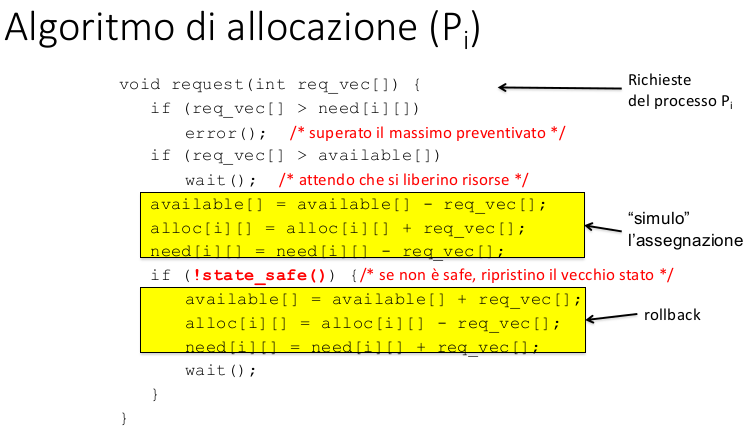
\includegraphics[width=1\textwidth]{banchiere1.png}
\end{center}

\begin{center}
    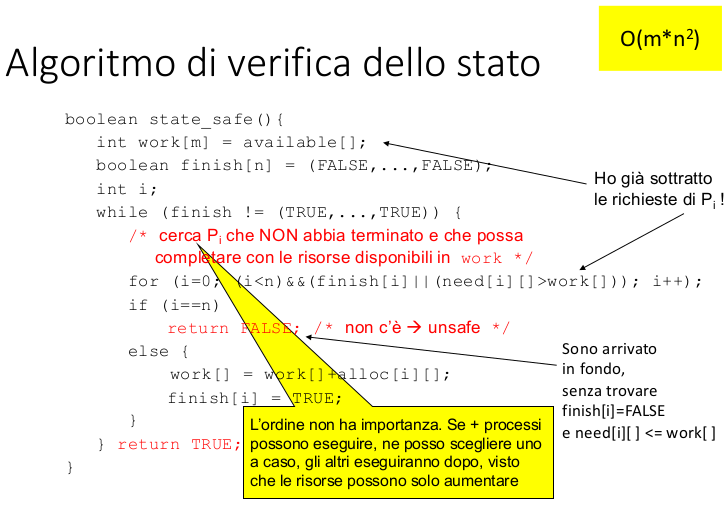
\includegraphics[width=1\textwidth]{banchiere2.png}
\end{center}
3) L'algoritmo di rilevazione permette che ci siano dei Deadlock, ogni tanto verifica che il sistema sia caduto in Deadlock
 in un metodo simile all'algoritmo del banchiere senza la necessità di conoscere la matrice max, verifica solo se il sistema è in 
 uno stato SAFE. Usa strutture dati simili a quello del banchiere.
 \begin{center}
     \begin{verbatim}
         int available[m]; //n° istanze di R_i disponibili
         int alloc[n][m]; //matrice allocazione corrente
         int req_vec[n][m]; //matrice di richiesta,
                            //stesse dimensione della max,
                            // è una max istantanea
     \end{verbatim}
 \end{center}
 \begin{center}
     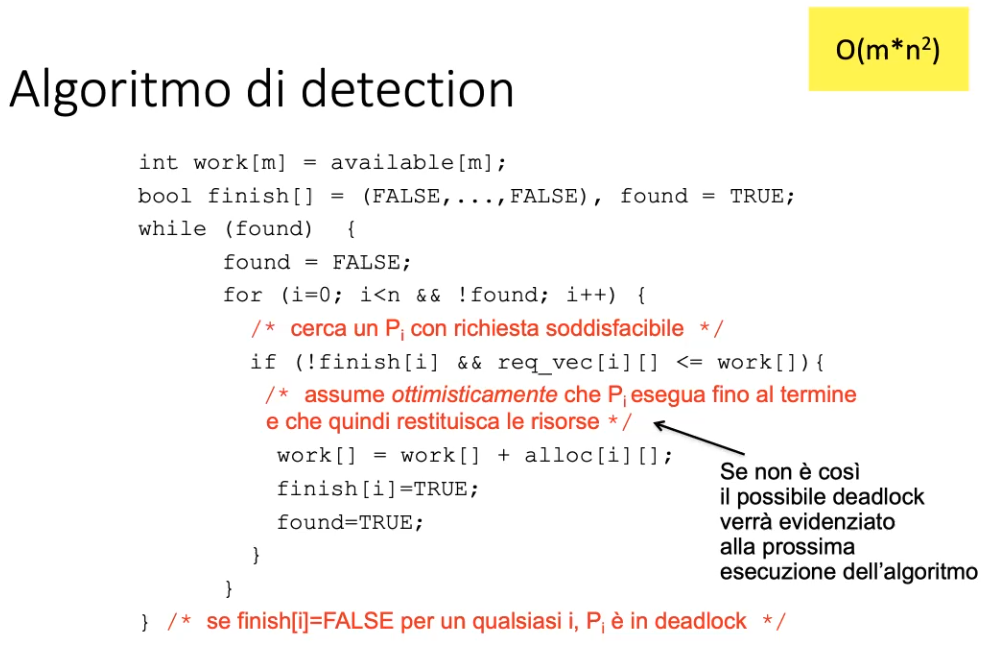
\includegraphics[width=1\textwidth]{detection.png}
 \end{center}
 Parte dal presupposto che tutti i processi siano bloccati,
 verifica se il singolo processo non ha finito e se le risorse che richiede siano inferiori a quelle disponibili.
  come trova un processo che può proseguire
  con la sua esecuzione significa che non si è in Deadlock, non verifica la situazione futura, solo quella attuale.
Esempio:
\begin{center}
    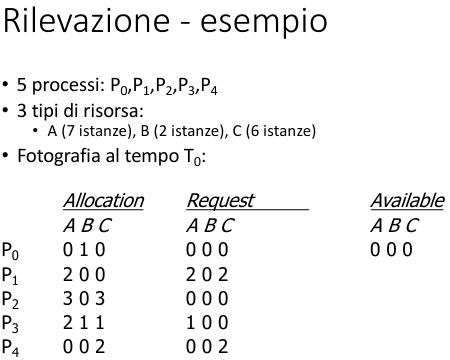
\includegraphics[width=1\textwidth]{detection2.png}
\end{center}
Usando l'algoritmo si passa man mano ogni singolo processo e si verifica se nello stato attuale può finire la sua esecuzione
 oppure è fermo a causa di un'attesa di risorse. Man mano che si trovano processi che possono concludere, si considerano 
 le risorse in loro possesso come possibili risorse future disponibili.

 L'algoritmo di rilevazione può essere lanciato:
 \begin{itemize}
     \item dopo ogni richiesta di risorsa
     \item ogni N secondi
     \item quando la percentuale di utilizzo della CPU cala sotto una soglia T
 \end{itemize}
 La prima è particolarmente costosa, non si fa prevenzione, ma si verifica sempre, che può essere problematico essendo 
 un algoritmo che può arrivare ad avere una complessità cubica. La terza opzione potrebbe non rilevare dei Deadlock causati da 
 piccoli gruppi di processi che non causano grossi cali d'uso della CPU.

 Quando ci si accorgerà del Deadlock si potrà:
 \begin{itemize}
     \item uccidere tutti o alcuni dei processi coinvolti
     \item prelazionare tutti i processi coinvolti
 \end{itemize}
 In entrambi i casi sarebbe un grosso danno, perché i processi hanno lavorato fino a quel momento  
 per niente.
 Per la prima, invece di uccidere tutti i processi si può scegliere di ucciderne uno alla volta in base  
 alle risorse allocate, a quante ne mancano, a quanto tempo mancava, etc e verificare dopo se il Deadlock 
 è tuttora presente o meno.
 La seconda possibilità invece porta il problema che prelazionare un singolo processo equivale quasi a ucciderlo 
 visto che non può continuare normalmente come prima, una possibile soluzione è il \textbf{rollback} che comporta
 un lavoro in precedenza eseguito dalla CPU per salvare uno stato in cui il processo non era bloccato.
 Successivamente questo potrebbe causare un fenomeno di starvation se si andrà a fare \textbf{rollback} dei soliti
 processi, in quel caso una possibile soluzione potrebbe essere quella di considerare il numero di \textbf{rollback}
 nei fattori di costo.

 \chapter{Gestione della memoria}

 Un processo ha bisogno sia di memoria RAM che di memoria di massa per poter lavorare. La memoria serve ai processi per
 via dell'uso del \textbf{Program Counter} da parte della CPU .
 Possono nascere svariati problemi nella gestione della memoria per i processi:
 \begin{itemize}
     \item l'allocazione della memoria dei singoli processi
     \item protezione dello spazio allocato
     \item condivisione dello spazio allocato
     \item gestione dello swap
     \item gestione della memoria virtuale
 \end{itemize}
 Ogni programma per essere eseguito deve essere messo in memoria e trasformato in processo, da quel momento la CPU
 preleverà istruzioni dalla memoria in base al \textbf{Program Counter}, questo può portare all'ulteriore prelievo di dati dalla
 memoria fino alla fine dell'esecuzione con l'eventuale scrittura in memoria del risultato, una volta che il processo terminerà
 la memoria verrà rilasciata.

 \paragraph{Come avviene il passaggio da programma a processo?}
 La trasformazione avviene tramite una trasformazione di indirizzi di memoria.
 \begin{center}
     \begin{verbatim}
         int x = 3;
     \end{verbatim}
 \end{center}
 non è altro che un riferimento a un indirizzo di memoria, quando il programma verrà eseguito, quell'indirizzo
 \textbf{simbolico} verrà tradotto in un indirizzo \textbf{fisico}.
 \paragraph{Chi compie questa trasformazione?}
 \begin{description}
     \item [il compilatore:] prende l'indirizzo \textbf{simbolico} e lo trasforma in una serie di indirizzi \textbf{rilocabili}
     ovvero che si possono posizionare da un'altra parte
     \item [il linker e/o il loader:] prendono l'indirizzo \textbf{rilocabile} e lo trasformano in indirizzo fisico assoluto
 \end{description}
 Possono essere coinvolti tutti o no, in base a come avviene la trasformazione.
 \begin{center}
     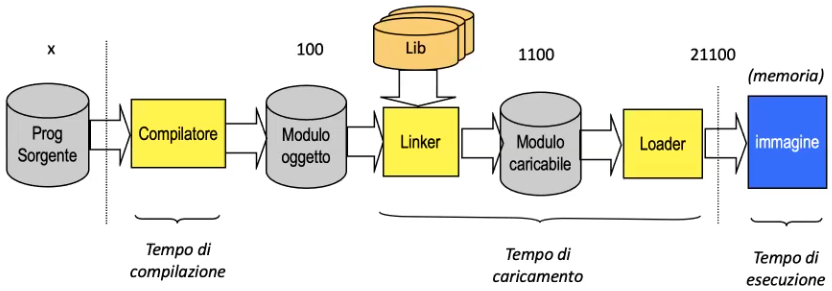
\includegraphics[width=1\textwidth]{trasformazione.png}
 \end{center}
La variabile X viene presa dal \textbf{compilatore} e trasformata da indirizzo \textbf{simbolico} a indirizzo \textbf{rilocabile}, viene
creato un modulo oggetto, in cui alla variabile viene assegnato un indirizzo di memoria, X non sarà più X, sarà l'area di memoria
all'indirizzo 100. Il \textbf{linker} collegherà l'indirizzo 100 con gli indirizzi delle eventuali librerie incluse nel programma,
ciò causerà la creazione di un modulo ricaribile in memoria. La X dall'indirizzo 100 sarà spostata all'indirizzo 1100 per fare spazio
alle eventuali librerie. Il modulo caricabile è quello che effettivamente verrà caricato in memoria dal \textbf{loader}. Il SO
assegnerà uno spazio all'interno della memoria tenendo conto dello spazio effettivamente occupato al momento. Eventualmente se
l'indirizzo 1100 fosse occupato, il SO potrà spostarlo a un altro indirizzo libero, fatto questo il processo verrà eseguito.
Se si troverà un'istruzione 
\begin{center}
    \begin{verbatim}
        int a = x + b;
    \end{verbatim}
\end{center}
vedendo che l'operando da prelevare è X, verrà ripescato dall'indirizzo di memoria, tale azione che collega indirizzi 
\textbf{simbolici} a indirizzi \textbf{fisici} viene denominata \textbf{binding degli indirizzi}.
\section{Tempi di compilazione}
\begin{description}
    \item[compile-time:] avviene a tempo di compilazione,in quel caso ci sarà solo il 
    \textbf{compilatore} che non può sapere se l'indirizzo che assegna al programma sia occupato o meno, di conseguenza 
    in caso in cui fosse occupato il programma semplicemente non verrà eseguito. Ciò funziona bene se la memoria è ottimizzata
    al massimo. Per cambiare la locazione del programma l'unica opzione sarà quellla di ricompilarlo.
    \item[load-time:]avviene a tempo di caricamento, il \textbf{loader} può notare che l'area di memoria in cui vuole
    caricare sia occupata e di conseguenza cambia l'area in cui andare a caricare. Il codice sarà rilocabile, anche se non permette
    di spostare il processo mentre è in esecuzione. Se cambiasse l'indirizzo di riferimento sarà necessario ricaricare.
    \item[run-time:]permette di spostare l'indirizzo di memoria allocato mentre il processo è in esecuzione, è necessario un 
    supporto hardware perché decisamente più efficiente. 
\end{description}
I primi due tipi di \textbf{binding} sono considerati \textbf{statici} mentre l'ultimo è considerato \textbf{dinamico}.

\section{Linking}

Può essere diverso indipendentemente dal tipo di \textbf{binding}.
\begin{description}
    \item[statico:] tradizionale, prima di mandare in esecuzione il processo, si è creato un'immagine di memoria con 
    tutte le librerie incluse.
    \item[dinamico:]il sistema viene preparato per accogliere un'immagine del codice e delle librerie, ma il linking vero e
    e proprio avverrà solo al momento dell'esecuzione, l'eseguibile sarà più piccolo perché non conterrà le librerie, ma solo 
    il loro riferimento.  
\end{description}

Un programma linkato staticamente occuperà una maggior memoria rispetto a un programma linkato dinamicamente, dal punto di vista
di caricamento il dinamico vince sullo statico, in quel caso gli stub creati dal linkato dinamico dovranno essere completati a 
\textbf{run-time} e ciò porterà il programma a essere più lento rispetto a quello linkato staticamente.

Ricapitolando:
\begin{description}
    \item[linking statico:]\begin{itemize}
        \item occupa maggior memoria
        \item lento nel caricamento
        \item veloce nell'esecuzione
    \end{itemize} 
    \item[linking dinamico:]\begin{itemize}
        \item occupa meno memoria
        \item più rapido nell'avvio
        \item più lento nell'esecuzione
    \end{itemize}
\end{description}

\section{Loading}

Lo stesso concetto di statico e dinamico può essere applicato al \textbf{loader}.
\begin{description}
    \item[statico:] tutto il codice viene caricato in memoria al tempo di esecuzione, quindi deve essere disponibile in 
    memoria prima di eseguire il programma
    \item[dinamico:] i moduli che servono al processo vengono caricati al primo utilizzo, se una parte non serve non verrà
    caricata di conseguenza 
\end{description}

Uno dei malus dello \textbf{statico} è la possibilità di programmi in cui una parte del codice non verrà mai eseguita (magari
per via di condizioni), non conviene di conseguenza caricare completamente il programma, in quel caso il loading \textbf{dinamico}
diventa decisamente più utile.

\section{Spazio di indirizzamento logico}

Consiste nello spazio visto dalla CPU quando esegue un processo, mappato su uno spazio di indirizzamento fisico in RAM. Il SO 
deve mappare indirizzi logici o virtuali su indirizzi fisici reali, quando si fa \textbf{binding} a \textbf{compile-time} o
\textbf{load-time} l'indirizzo logico e fisico coincidono. Invece con un \textbf{binding} a \textbf{run-time} l'indirrizzo
logico generato dalla CPU potrebbe non coincidere con quello fisico presente in RAM, tutto ciò viene sempre gestito dal
SO. Una gestione dinamica come questa ha un costo, ovvero il tempo che ci mette la MMU (Memory Management Unit) che tiene 
conto del riferimento tra indirizzo logico a quello fisico a tradurre la richiesta.

La MMU può essere composta da un registro e un sommatore che somma gli indirizzi logici con un offset, potrebbe essere problematico
con processi che dovrebbero essere divisi all'interno dello spazio di memoria.

\chapter{Schemi di gestione della memoria}

\section{Allocazione contigua}

L'immagine di memoria del processo sarà tutto allocata in un'area contigua per l'appunto, senza buchi in mezzo. Per gestire tale
l'allocazione in questo modo esistono delle varianti:

\subsection{Partizioni fisse}

La memoria è divisa a blocchi, ciascun blocco con una determinata
    dimensione che rimarrà fissa per sempre, tra di loro possono differire in dimensione, ma rimarranno fisse. Il processo che arriva
    verrà posizionato nella prima partizione che permette di contenerlo. Un contro è che se un blocco viene occupato solo in 
    parte, quella libera sarà sprecata, perché il blocco è fisso e non può essere partizionato. Esistono delle opzioni:

    \begin{itemize}
        \item un'unica coda di attesa, con i processi in fila e come si libera uno spazio il processo in testa verificherà
        se riesce a entrarci o meno
        \item tante code, una per partizione, il SO fa un preselezione del processo che verrà messo nella coda più adatta a lui
    \end{itemize}

    Entrambe hanno vantaggi e svantaggi, una coda per partizione causerà la possibilità di avere delle code vuote e altre piene, 
    in quel caso si avrebbe tanta memoria sprecata e pochi processi in coda. Va bene solo nel caso in cui il carico dei vari processi
    è ben distribuito e di varie dimensioni. Se tutte le code fossero piene, sarebbe ottimale per l'uso della memoria.

    Nell'alternativa con un'unica coda, la gestione sarà più complicata, perché un processo troppo grande per stare in partizioni
    troppo piccole rimarrebbe in attesa in caso di algoritmo FCFS, bloccando tutti gli altri processi dietro di lui che 
    potrebbero entrare nelle partizioni libere. Una scansione della coda quando si libera una partizione risolve il problema, ci 
    sono due varianti
    
    \begin{description}
        \item[Best-fit:] scansiona tutta la coda scegliendo quello più adatto alla partizione che si è liberata
        ovvero quello che si avvicina a occuparla maggiormente, se la coda è molto lunga il tempo impiegato sarà decisamente
        elevato;
        \item[Best-available-fit:] viene scelto il primo processo che può stare nella partizione che si è liberata, non minimizza
        lo spreco, perché potrebbe esserci un processo che occuperebbe meglio la partizione.
    \end{description}

Lo schema della MMU con un allocazione contigua a partizioni fisse è il seguente:

\begin{center}
    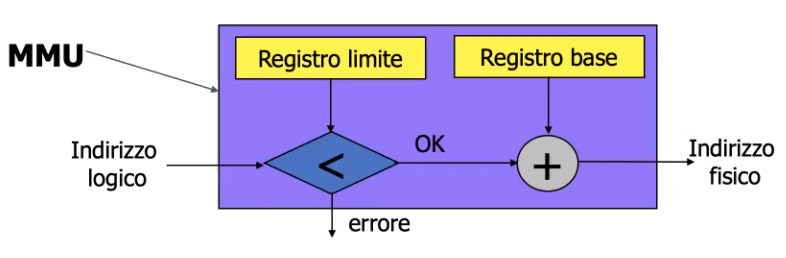
\includegraphics[width=1\textwidth]{mmu_partizioni_fisse.png}
\end{center}

Pro e contro:

\begin{description}
    \item[Pro:] semplicità, il SO deve solo tenere traccia di una tabella in cui si definisce in quale partizione andrà il processo
    \item[Contro:] il livello di multiprogrammazione è vincolato dal numero di partizioni, inoltre c'è uno spreco di memoria causato
    dalla frammentazione:
    
    \begin{description}
        \item[Interna:] causata dall'assegnamento di un processo a una partizione che non viene occupata al 100%
        \item[Esterna:] la somma della parte libera di partizioni parzialmente occupate potrebbe essere grande a sufficienza
        per un processo che invece sarà costretto ad attendere 
    \end{description}
    la frammentazione riduce l'efficacia nell'uso della memoria, la tecnica con partizioni fisse soffre di entrambe, è più adatta per
    processi delle dimensioni giuste ed esatte alle partizioni che si vogliono occupare, quindi più verso i sistemi embedded.
\end{description}

\subsection{Partizioni variabili}

Il processo che arriva in memoria si prenderà una fetta di memoria grande esattamente quanto lo spazio che occuperebbe.
La frammentazione esterne rimarrà, esempio:

\begin{itemize}
    \item si crea una partizione da 100, una da 50, una da 30 e una da 20
    \item si libera quella da 50 e da 20
    \item un processo che occupa 70 potrebbe entrare se le posizioni da 50 e 20 venissero sommate, ma non si può a causa dell'allocazione contigua
\end{itemize}

Si genera un effetto a "groviera". 
 
\subsection{Tecnica del Buddy System}

Un compromesso tra partizioni fisse e variabili, ovvero
ha partizioni fisse, ma anche variabili, le dimensioni 
non sono customizzate, ma non rimangono fisse. Bisogna 
immaginare la memoria un blocco fisso, come arriva un
processo parte il sequente schema:  

\begin{SCfigure}[50][h!]
    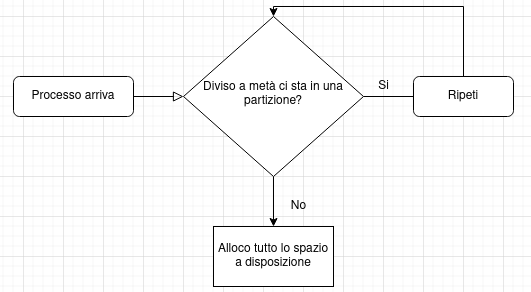
\includegraphics[width=0.5\textwidth]{buddy_system.png}
    \caption{Flowchart Buddy System}
\end{SCfigure}

Questo crea liste di blocchi liberi in base alla dimensione,
al processo successivo si andrà a guardare nella lista
se ci sta altrimenti si ripete la divisione.

\section{Paginazione}

Elimina totalmente la frammentazione esterna. La memoria fisica
viene suddivisa in tante piccole aree della stessa dimensione detti \textbf{frame}.
Lo spazio di allocazione non deve essere contiguo, al processo 
che arriva si daranno piccole aree fino a occupare tutte 
quelle necessarie. Il processo viene diviso,
quando un processo dovrà essere eseguito in CPU, SO dovrà
ricomporlo, quindi occorre una mappa delle locazioni.

La CPU è a conoscenza degli indirizzi logici, la memoria
logica viene divisa in blocchi della stessa dimensione le \textbf{pagine}, il SO 
trasforma le pagine in frame.
Entra in aiuto una tabella delle pagine, ovvero una mappa
della memoria specifica per ogni singolo processo, attraverso
la quale il SO riesce a tradurre l'indirizzo logico che serve alla 
CPU in un indirizzo fisico e recuperare di conseguenza le 
informazioni necessarie.

Esempio:
\begin{itemize}
    \item dimensione della pagina = 1KB
    \item dimensione del programma = 2.3KB
    \item saranno necessarie 3 pagine, dell'ultima si userà solo 0.3KB
\end{itemize}
Come si può notare sarà ancora possibile la frammentazione
interna.

\paragraph{Come avviene la ricerca nella tabella delle pagine?}
L'indirizzo logico richiesto dalla CPU è composto dal numero
di pagina e da un offset, SO tramite il numero di pagina 
andrà alla ricerca nella tabella delle pagine del processo
in questione, una volta trovato otterrà l'altra metà di 
indirizzo fisico da sommare all'offset per ottenere 
l'indirizzo fisico effettivo in memoria.

Ovviamente la tabella risiede in memoria, ed è come già detto 
specifica del processo. Nei registri della CPU sarà presente 
la locazione della tabella e anche la sua lunghezza, a ogni context 
switch tale valore viene aggiornato.

Questo causa un doppio accesso alla memoria: uno per 
la tabella delle pagine e uno per l'istruzione/dato necessari, per 
questo si usa una cache dedicata, \textbf{Translation look-aside table}(TLB), 
servirà a evitare il doppio accesso in memoria, in caso 
di cache miss, ovvero TLB non sarà in possesso della pagina, si 
dovrà per forza fare il doppio accesso in memoria.

Il costo effettivo di accesso in memoria sarà dato dalla 
somma del cache hit all'accesso in memoria:
\[
    \overbrace{(T_{MEM} + T_{TLB})\alpha\textrm{(parametro)}}^{\textrm{cache hit}} + \overbrace{(2T_{MEM} + T_{TLB})(1 - \alpha)}^{\textrm{accesso in memoria}}
\]

La tabella delle pagine è utile anche per altro:
\begin{description}
    \item[Bit di validità:] identifica se l'area di memoria 
    è stata mappata per il processo o no;
    \item[Caratteristiche:] un bit che comunica se la pagina
    è solamente leggibile o no, per esempio il codice di una programma
    è in sola lettura, oppure se la pagina sia eseguibile o meno.
\end{description}

\paragraph{Quanto è grande una tabella della pagine?}
La dimensione è stabilita in base alla memoria massima e alla configurazione,
ovvero quanto grande è ogni frame della memoria. In un ipotetico spazio di indirizzamento
virtuale grande $2^{64}$, se ogni pagina avesse una dimensione di 4KB ovvero $2^{12}$ potrei 
avere un numero di frame in memoria corrispondente al rapporto tra la memoria indirizzabile totale e
la dimensione della singola pagina. 
\[
    2^{64} / 2^{12} = 2^{52}
\]
Un numero decisamente enorme che occuperebbe una grossa fetta della RAM da moltiplicare per il 
numero di processi attivi. Si possono usare due metodi per evitare ciò:
\begin{itemize}
    \item una tabella delle pagine invertita;
    \item oppure la paginazione multilivello.
\end{itemize}

\subsection{Tabella delle pagine invertita}
Una tabella unica nel sistema e non per processo, indicizzata per frame che contiene:
\begin{itemize}
    \item l'indirizzo virtuale della pagina che occupa quel frame
    \item informazioni sul processo che usa la pagina
\end{itemize}
Il tempo di traduzione degli indirizzi cresce perché non sarà più una ricerca per indice, ma per contenuto. Perché 
la tabella è indicizzata per frame, mentre la CPU richiederà per pagina, il SO dovrà scorrere la tabella alla ricerca della 
pagina e solo così otterrà il frame corrispondente che sarà l'indice del contenuto. Questo viene facilitato tramite una struttura 
a tabella hash, invece di usare una ricerca lineare. Cambia come viene generato l'indirizzo richiesto dalla CPU, sarà diviso in tre parti:
\begin{itemize}
    \item offset;
    \item numero di pagina;
    \item PID del processo.
\end{itemize}

Con il numero di pagina e il PID ho la chiave per la tabella hash, così da ottenere il valore ricercato per la traduzione ovvero
l'indice, perché la tabella è indicizzata per frame!

\subsection{Paginazione multilivello}
Viene paginata anche la tabella delle pagine, quindi spezzettata per fare in modo che alcuni pezzi non siano in RAM, lasciando 
spazio libero in memoria per altro di più utile. Questa azione può essere ripetuta anche per i pezzi delle tabella delle pagine, 
per più livelli di paginazione.  Esempio:
\begin{itemize}
    \item indirizzo logico a 32 bit;
    \item dimensione della pagina = 4K = $2^{12}$;
    \item 12 bit per offset(d);
    \item 20 bit per numero di pagina:
    \begin{itemize}
        \item 10 bit per l'indice della tabella delle pagine esterna;
        \item 10 bit per l'offset all'interno della pagina della tabella delle pagine interna.
    \end{itemize}
\end{itemize}
Il costo per un accesso in memoria con una paginazione multilivello cambia di conseguenza nello speficico,
l'accesso in memoria sarà moltiplicato per $n + 1$ livelli di paginazione:
\[
    (T_{MEM} + T_{TLB})\alpha + ((n + 1)T_{MEM} + T_{TLB})(1 - \alpha)
\]
Il $+1$ causato dall'accesso al dato.

\section{Segmentazione}
Il problema della paginazione è che lo spezzettare a blocchi il processo viene fatto senza rispettare la struttura dati 
creata dal compilatore, sarebbe più utile avere pagine contenenti blocchi interi utili: una pagina con il main, una per le 
funzioni, etc\dots Finché la pagina ha una dimensione fissa questo non si può ottenere, la \textbf{segmentazione} è analoga alla 
paginazione, ma non si vincola più alla dimensione di una pagina fissa. Dal punto di vista di SO, avremo una tabella dei segmenti 
che verranno tagliati a dimensione variabile. Un segmento di dimensioni variabili torna ad avere la problematica dell'allocazione 
contigua, ovvero che non può essere messo dovunque, ma in blocchi unici. Nella tabella dei segmenti, ogni entry conterrà oltre 
che all'indirizzo base del segmento anche la sua dimensione, che precedentemente non era necessaria con le pagine. 
\paragraph{Come cambia la traduzione?}
La CPU richiederà un indirizzo composto da una parte segmento e una parte offset, l'offset verrà analizzato, per verificare se 
va oltre la dimensione del segmento o se rimane al suo interno (ecco da cosa viene causato il segmentation fault). La parte di offset
verrà sommata al valore restituito dalla tabella dei segmenti, che ricordiamo contenere la dimensione del segmento e la base da sommare
eventualmente all'offset. Esempio di traduzione:
\begin{center}
    \begin{tabular}{| c | c | c |}  
        \hline
        Segmento & Limite & Base \\
        \hline
        0 & 600 & 219 \\
        \hline
        1 & 14 & 2300 \\
        \hline
        2 & 100 & 90 \\
        \hline
        3 & 580 & 1327 \\
        \hline      
    \end{tabular}
\end{center}

A ogni segmento si avrà appunto il suo limite e la sua base, per esempio

\begin{itemize}
    \item se venisse richiesto il segmento $0$ e l'offset $430$ 
    si controlla il segmento $0$, si nota che l'offset $430$ è all'interno del limite di conseguenza l'indirizzo fisico sarà dato da: 
    offset + base = $649$.
    \item segmento $1$ offset $20$? segmentation fault perché $20$ è superiore al limite $14$
\end{itemize} 

La segmentazione mi garantisce di gestire ancora meglio tutti gli aspetti visti nella paginazione, perché adesso avrò la certezza
che il contenuto del segmento sarà omogeneo.

\paragraph{Svantaggi della segmentazione}

Torna il problema della frammentazione esterna, la pagina può essere messa in qualunque spazio, perché sono tutti uguali, 
mentre il segmento essendo variabile ma richiedendo un'allocazione contigua non può e ciò causa la frammentazione esterna. 
Una possibile soluzione al problema è l'unione della paginazione e della segmentazione, segmento il processo e ogni segmento lo 
pagino, segmentandolo prima mantengo l'unità logica che verrà paginata omogeneamente in multilivelli.

\section{Paginazione vs Segmentazione}

Vantaggi della paginazione:
\begin{itemize}
    \item non esiste frammentazione, a parte una piccola frammentazione interna;
    \item l'allocazione dei frame non richiede algoritmi specifici;
\end{itemize} 
Svantaggi della paginazione:
\begin{itemize}
    \item non mantiene l'omogeneità;
\end{itemize}
Vantaggi della segmentazione:
\begin{itemize}
    \item omogeneità;
    \item associazione di protezione/condivisione ai segmenti;
\end{itemize} 
Svantaggi della segmentazione:
\begin{itemize}
    \item richiede degli algoritmi di allocazione dinamica dello spazione, essendo i segmenti variabili;
    \item reintroduce la problematica della frammentazione esterna;
\end{itemize}

Unendole si porteranno dietro i vantaggi di ciascuna limitando gli svantaggi.

\section{Segmentazione paginata}

L'indirizzo logico sarà composto da segmento e offset, il numero di segmento verrà sommato al valore all'interno \textbf{Segment Table Base Register} (indica dove si trova la tabella dei segmenti all'interno della memoria) 
per andare a indicizzare la tabella dei segmenti. All'interno della tabella dei segmenti si troverà la lunghezza del segmento e 
la \textbf{Page Table Base} in cui si troverà l'indirizzo di locazione della tabella delle pagine specifica di quel segmento. 
L'indirizzo verrà combinato con l'offset, che è composto da due parti, una che indica il numero di pagina e una che indica 
l'offset effettivo. Il numero di pagina verrà sommata al \textbf{Page Table Base Register} per recuperare la riga effettiva della 
tabella delle pagine, una volta indicizzata la riga in questione, si sommerà il valore del frame all'offset effettivo e si farà 
l'accesso alla memoria per recuperare il dato necessario. 

\chapter{Memoria virtuale}

\section{Motivazioni}

L'immagine di memoria di un processo è davvero necessaria che sia \textbf{tutta} caricata in RAM? In generale no, serve solo una parte,
ovvero quella che rappresenta la località spazio temporale necessaria. Quella che non serve verrà lasciata sul disco, 
questo permetterà di lasciare spazio libero in memoria per altre immagini di memoria più utili e avvantaggiare la multiprogrammazione.
Lo spazio logico sarà più grande dello spazio in memoria, perché sarà composto dalla somma di tutte le immagini dei processi che 
saranno in parte in RAM e in parte sul disco. 

\section{Paginazione su domanda}

Una pagina si troverà in memoria solo quando necessaria. I vantaggi sono i seguenti:
\begin{itemize}
    \item meno memoria occupata da ogni processo;
    \item se il livello di multiprogrammazione fosse troppo alto, l'eventuale swap out verrà fatto solo a una parte delle pagine riducendo i tempi di I/O;
\end{itemize}

Per poter implementare occorre sapere se la pagina richiesta dalla CPU sia valida o no, entra in gioco il bit di validità presente
nella tabella delle pagine. Quel bit segnalerà se la pagina si trova in RAM, su disco oppure se la pagina non si trova 
nell'intervallo di memoria. Quando una pagina è mappata su un frame che non si trova in RAM, bit validità = 0, avviene un \textbf{page fault}.
Quindi:

\begin{enumerate}
    \item controllando sulla tabella delle pagine risulterà che la pagina è invalida, non è in RAM, di conseguenza sarà su disco;
    \item parte un interrupt, il \textbf{page fault};
    \item il S.O. verificherà che la pagina si trovi nella parte di disco dedicata alla funzione di RAM, (\textbf{Backing Store} o \textbf{Area di Swap});
    \item localizza la pagina e la riporta nella memoria, cercherà un frame e caricherà la parte di memoria recuperata;
    \item reset della \textbf{page table} per indicare che ora la pagina è in memoria con annessa aggiunta dell'indirizzo e modifica del bit validità;
    \item il processo verrà rimesso in ready queue per essere pronto all'esecuzione.
\end{enumerate}

Questo avviene a ogni \textbf{page fault}. 

\subsection{EAT di un Page Fault}

Introduciamo un parametro p (tasso di page fault), che vale in questo intervallo $0 \le p \le 1$, dove 

\begin{itemize}
    \item p = 0, nessun page fault;
    \item p = 1, ogni acceso è un page fault.
\end{itemize}

\[
    EAT = (1 - p) * t_{mem} + p * t_{\textrm{page fault}}
\]

La parte $p * t_{\textrm{page fault}}$ è la moltiplicazione tra la percentuale di page fault e il tempo richiesto per recuperare il 
dato su disco, mentre $t_{mem}$ è il tempo di accesso alla memoria tramite il meccanismo di gestione dell'allocazione di 
memoria ai processi. Il $t_{\textrm{page fault}}$ è composto dalla gestione dell'interrupt che arriva, il context switch per 
permettere al S.O. di gestire la situazione, torna al processo che era stato interrotto (context switch).

\begin{itemize}
    \item gestione dell'interrupt (primo context switch);
    \item swap in, lettura della pagina mancante da disco a memoria;
    \item costo di riavvio del processo (secondo context switch);
    \item (opzionalmente) swap out della pagina che devo estrarre per fare spazio a quella richiesta.
\end{itemize}

Ci sono ben due context switch.

\subsection{Rimpiazzamento delle pagine}

In caso di assenza di frame liberi in cui mettere la pagina recuperata:

\begin{itemize}
    \item tramite un algoritmo specifico di rimpiazzamento delle pagine si trova una pagina da sostituire;
    \item avviene lo swap su disco della pagina sostituita;
    \item swap dell'altra pagina nel frame dal disco;
    \item modifica le tabelle (tabella delle pagine e bit di validità);
    \item ripristino dell'istruzione che ha causato il page fault.
\end{itemize}

Rimpiazzare una pagina costa il doppio di una normale gestione del page fault. Per questo entra in gioco l'utilità del \textbf{dirty bit}
ovvero un bit che specifica se la pagina è stata modificata mentre si trovava in memoria o meno, in caso di una modifica occorre
ricaricarla su disco. Rimpiazzare una pagina che non è stata modifica costa meno, perché si può semplicemente sovrascrivere.

\subsection{Algoritmi di rimpiazzamento delle pagine}

Obiettivo: minimizzare il tasso di page fault, dipenderà dalla scelta delle pagine da caricare in memoria. Un metodo è l'uso 
di una stringa di riferimenti. Ipotizzando pagine grandi 100 byte, la stringa sarà composta dalla cifra delle centinaia delle 
pagine che verranno richieste. Esempio: 

\begin{itemize}
    \item indirizzi generati: 100, 604, 128, 130, 256, 260, 264, 268;
    \item la stringa di riferimento sarebbe composto da: 1, 6, 1, 1, 2 ,2, 2, 2;
    \item in realtà sarà composta da: 1, 6, 1, 2. Perché il page fault sarà possibile con la prima pagina, sicuramente non con quelle successive.
\end{itemize}

\subsection{Algoritmo FIFO}

Prima pagina che carico sarà la prima scelta a essere rimossa per liberare  eventualmente spazio, non è adatto nè per lo scheduling 
nè per la gestione della memoria. Può causare l'anomalia di Belady, ovvero aumentando la disposizione di frame in memoria potrebbero 
aumentare i page fault diversamente da quello che ci si aspetterebbe.

\begin{figure}[h!]
    \centering
    \subfloat[][\textbf{\emph{Esempio con algoritmo FIFO, causa 15 page fault}}]
    {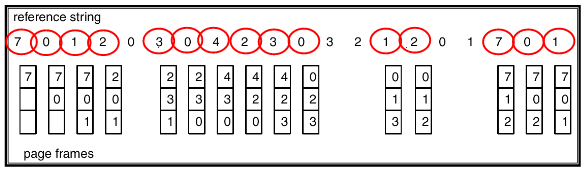
\includegraphics[width=0.5\textwidth]{FIFO.png}}\quad
    \subfloat[][\textbf{\emph{Anomalia di Belady, all'aumentare dei frame aumentano i page fault}}]
    {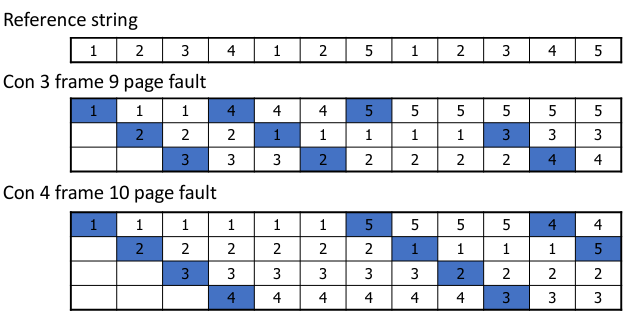
\includegraphics[width=0.5\textwidth]{belady.png}}
\end{figure}

\subsection{Algoritmo Ideale}

L'\textbf{algoritmo ideale}, dovrebbe essere in grado di scegliere la pagina che non userò per più tempo, garantendo che per un po'
 non avrò page fault.

\begin{SCfigure}[50][h!]
    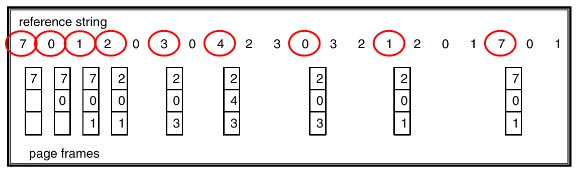
\includegraphics[width=0.5\textwidth]{ideale.png}
    \caption{Esempio di algoritmo ideale}
\end{SCfigure}

\subsection{Algoritmo LRU}

L'algoritmo \textbf{Least Recently Used}, approssima un possibile algoritmo ideale guardando al passato, rimpiazza la pagina
che non viene utilizzata da più tempo.

\begin{SCfigure}[50][h!]
    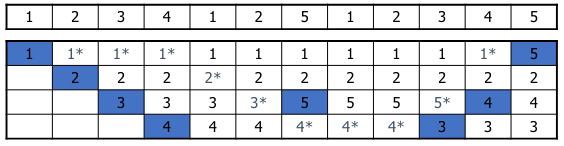
\includegraphics[width=0.5\textwidth]{LRU.png}
    \caption{Esempio di algoritmo LRU, uso dell'asterisco per indicare la pagina meno utilizzata da più tempo}
\end{SCfigure}

Lo si implementa tramite un contatore, all'interno si salverà il time stamp cioè il clock di sistema, indica da quanto non viene 
usata una pagina, il tutto verrà memorizzato nella tabella delle pagine. Inoltre quando avviene un page fault, sarà necessario far 
partire una ricerca tra tutte le pagine per vedere quale ha il time stamp più vecchio. Il tutto è decisamente costoso perché appunto 
sarà necessario avere il time stamp di tutte le pagine e successivamente bisognerà controllarle tutte alla ricerca di quelle più 
vecchio.

Una possibile approssimazione per risparmiare spazio e tempo perdendo un po' di precisione è tramite l'uso dello stack. Si evita di 
memorizzare il clock per ogni pagina, ma si crea una pila, uno stack in cui si tiene un ordine di accesso. In fondo sarà presente 
la pagina più vecchia, man mano che viene utilizzata si metterà in cima, trovando in fondo la meno usata e in cima la più usata. Sarà
comodo perché la vittima è sempre quella in fondo, ma scomodo perché bisognerà passare l'intero stack alla ricerca della pagina 
da mettere in cima.

\begin{center}
    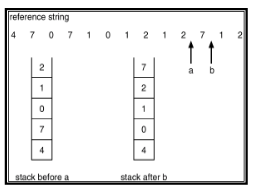
\includegraphics[width=0.7\textwidth]{LRU_approx.png}
\end{center}

Un'altra approssimazione potrebbe basarsi sui i bit di reference, alla pagina se ne assocerebbero di meno, con un limite inferiore 
uguale a 1, mentre il massimo il numero di bit necessari a memorizzare il time stamp. Si userà per individuare le pagina da eliminare
in caso di necessità, quindi varrà 0 o 1, se 0 verrà eliminata.

Un'ulteriore approssimazione è tramite l'algoritmo dell'\textbf{orologio} o algoritmo \textbf{secondo chance}. Al posto delle ore 
si metteranno i numeri di pagina, la prima e la seconda lancetta si muoveranno senza mai modificare l'angolo tra di loro. Come 
la prima lancetta raggiungerà una pagina, metterà il bit di reference a 0, quindi un unico bit per ogni pagina. La pagina ha tempo 
tanto quanto l'angolo formato tra le lancette per tornare a 1, in caso contrario significherà che quella pagina non è stata riferita,
nel momento in cui servirà una "vittima" da rimuovere, come passerà la seconda lancetta verrà scelta quella pagina.

Una quarta opzione si basa non più sul tempo, ma sulla frequenza in cui una pagina verrà riferita. Qui si avranno due opzioni:
\begin{itemize}
    \item Algoritmo LFU (\textbf{Least Frequently Used}), conto quante volte viene riferita una pagina, nel caso in cui mi serva 
    una vitta sceglierò quella con il conteggio più basso;
    \item Algoritmo MFU (\textbf{Most Frequently Used}), l'esatto opposto, ipotizza che la pagina con meno riferimenti sia stata 
    caricata da poco e che potrebbe venire utilizzata maggiormente in futuro.
\end{itemize}

\chapter{Allocazione dei frame}

Quanti frame assegnare a un processo? Occorre sapere qual è il numero minimo di frame che si possono assegnare per dargli la garanzia 
che riesca a eseguire un'istruzione alla volta. Quanti frame richiede un'istruzione? Potrebbe richiederne uno come anche due nel 
caso in cui l'istruzione sia a cavallo di due pagine, a questi bisogna aggiungere gli eventuali operandi che in base all'architettura 
se fossero tre, potrebbero essere anche loro  su due pagine diverse arrivando a un totale possibile di 8 frame necessari. Il minimo 
è dato dal massimo numero di indirizzi specificabili da un'istruzione, che cambia da architettura ad architettura.

Dal minimo si può ovviamente salire, ma di quanto? Ci può essere anche qui un'allocazione \textbf{fissa} e un'allocazione \textbf{variabile}. 

\begin{description}
    \item[Allocazione fissa:] ogni processo riceve un numero di frame definito, non per forza uguale per tutti, ma che non varia una volta definito;
    \item[Allocazione variabile:] il numero di frame di un processo può variare durante la sua esecuzione, è decisamente più difficile da gestire; 
\end{description}

\section{Allocazione fissa}

Si divide in due ulteriori categorie:

\begin{description}
    \item[In parti uguali:] i frame vengono assegnati in maniera equa a ogni processo, anche se un processo ne avrebbe bisogno di un numero maggiore;
    \item[Proporzionale:] in base alla grandezza in frame dei processi richiedenti i frame disponibili vengono assegnati in maniera proporzionale;  
\end{description}
Un contro della proporzionale è che un processo che richiede molti frame in realtà poi all'interno a righe di codice che gli portano 
a dover usare molti frame in meno rispetto a quella che sembrava inizialmente. 

\section{Allocazione variabile}

Una soluzione migliore, allocare a runtime è decisamente meglio, ma è molto difficile da gestire. Ci sono due possibili soluzioni:
\begin{itemize}
    \item tramite calcolo del \textbf{working set};
    \item tramite calcolo del PFF (\textbf{Page Fault Frequency});
\end{itemize}

\subsection{Working set}

Segue il principio di località, i frame verranno assegnati in base alla località. Come lo misuro? 

\begin{center}
    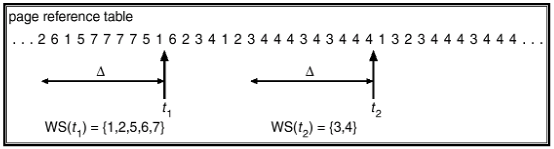
\includegraphics[width=0.5\textwidth]{working_set.png}
\end{center}
Periodicamento, al tempo $t_1$, $t_2$, etc..., si andrà a guardare a quante pagine ci si è riferiti negli istanti di tempo ovvero 
$\Delta$, all'istante $t_1$ il working set è di 5 pagine, ma all'istante successivo come si può vedere calerà a 2 pagine. In base a ciò
vengono assegnati i frame. Sarà fondamentale scegliere il parametro $\Delta$, troppo piccolo diventa poco significativo, troppo 
grande potrebbe essere a cavallo di due località. 

Cosa succede se la somma dei working set richiede un numero di frame maggiori di quelli a disposizione? Si verifica il fenomeno del 
\textbf{thrashing}, il SO si accorge che l'uso della CPU è sceso e ci sono molti processi in coda per fare accesso al disco e fare 
swap in e swap out. Una cattiva gestione porterebbe a fare entrare pronti altri processi, che avrebbero necessità
di memoria e di conseguenza tale memoria verrebbe rimossa a quelli già presenti, i quali vedranno i pochi frame a loro disposizione 
calare ulteriormente e di conseguenza richiederebbero ulteriori swap in e swap out e ciclicamente nuovi processi che entrano e 
ulteriori frame rimossi fino a un blocco totale. 

\subsection{Page Fault Frequency}

\begin{center}
    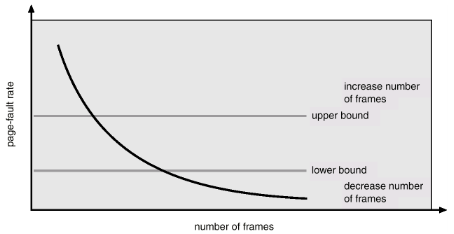
\includegraphics[width=0.5\textwidth]{pff.png}
\end{center}

L'obiettivo è di mantenere tutti i processi nella fascia 
intermedia tra upper bound e lower bound, il SO 
farà scelte per fare in modo che se ci sono processi 
sotto la soglia lower bound, gli toglierà dei frame perché 
il numero di page fault è molto basso, quindi potrà assegnare 
frame ai processi che superano la soglia di upper bound. 

\chapter{Memoria secondaria}

Necessaria per implementare la memoria virtuale e per memorizzare 
a lungo termine dati e programmi necessari. Diventa rilevante 
il concetto di tempo di accesso al disco, dipende da tre 
parametri:
\begin{itemize}
    \item \textbf{Seek Time}, tempo di spostamento della testina, meccanico, parte più lenta;
    \item \textbf{Latency Time}, tempo di attesa che il disco sottostante porti il settore di interesse sotto la testina, il disco ruota continuamente;
    \item \textbf{Transfer Time}, tempo necessario per spostare i dati da disco a controllore o viceversa.
\end{itemize}
Essendo il Seek Time il momento che fa perdere pià tempo in 
assoluto, conviene muoversi a cilindri lungo i dischi, così 
da non dover spostare la testina, ma bisogna anche considerare 
che non si riesce a memorizzare un file tutto contiguo.
Inolte poichè il disco è uno, ma i processi che leggono e scrivono
sono tanti, il SO riceverà molte richieste di lettura 
e scrittura su zone diverse del disco.

Queste problematiche svaniscono tramite l'uso di dispositivi
a stato solido, perché non ci sono più componenti meccaniche 
ma prettamente elettroniche.

\section{Scheduling degli accessi a disco}

Il disco è diviso in piatti concentrici, suddiviso in 
tracce e a loro volta suddivise in settori della stessa 
dimensione. Dal punto di vista logico come un vettore di 
elementi, un array di blocchi ordinati, tutti della stessa 
dimensione. Quando avviene un accesso al disco, ci sarà una 
coda di richieste con indirizzi e blocchi che indicano dove 
devono essere fatti e annessa quantità di dati da leggere 
o scrivere. 

Il SO ragiona in termini di costi ed efficacia per decidere
riguardo gli accessi. Esempio:
\begin{itemize}
    \item disco con 200 intervalli di valori ammissibili [0, 199];
    \item la testina di lettura e scrittua si trova sulla testina 53;
    \item le richieste di accesso sono per i valori: 98, 183, 37, 122, 14, 124, 65 e 67;
\end{itemize}
Applicando il meccanismo \textbf{FIFO}, la testina si sposterà a 
zig zag per eseguire tutti gli accessi.
\begin{center}
    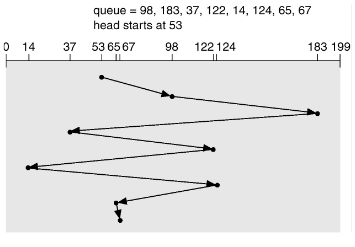
\includegraphics[width=0.5\textwidth]{zigzag.png}
\end{center}
Lo spostamento totale finale sarà di 640 tracce.

Una prima soluzione sarebbe quella di spostarsi verso la 
zona più vicina a quella in cui ci si trova, implementando 
l'algoritmo \textbf{SSTF} (Shortest Seek Time First), riduce 
lo spostamento della testina rispetto alla posizione attuale.
Questo algoritmo è decisamente ottimo rispetto al \textbf{FIFO}, 
ma non il migliore.
\begin{center}
    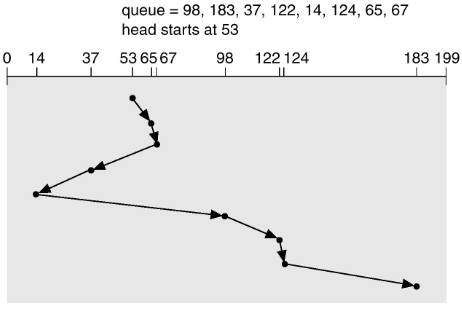
\includegraphics[width=0.5\textwidth]{sstf.png}
\end{center}
Se l'elenco di richieste accesso in lettura e scrittura fosse 
stabile, andrebbe bene, ma durante l'accesso al primo blocco
molto probabilmente arriverebbero altre richieste di accesso, 
quindi la coda di richieste è in continup aggiornamento.

Una possibile alternativa a questa è l'implementazione 
dell'algoritmo dell'ascensore o \textbf{SCAN}. Si sposta 
da un'estremità all'altra servendo tutto quello che si trova 
in mezzo.
\begin{center}
    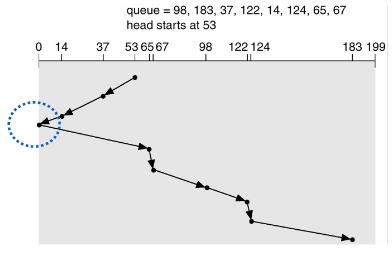
\includegraphics[width=0.5\textwidth]{scan.png}
\end{center}
Tale algoritmo si può migliorare, per esempio lo spostamento
nella traccia 0 non ha senso siccome non sono avvenute richieste 
minore della 14.

L'algoritmo \textbf{C-SCAN} o algoritmo dello spalatore 
di neve è simile allo SCAN, ma la differenza sta che una
volta raggiunta l'ultima traccia, ritorna alle tracce iniziali 
che molto probabilmente saranno state richieste dai processi.
Il tutto ovviamente senza servire le eventuali richieste 
intermedie.
\begin{center}
    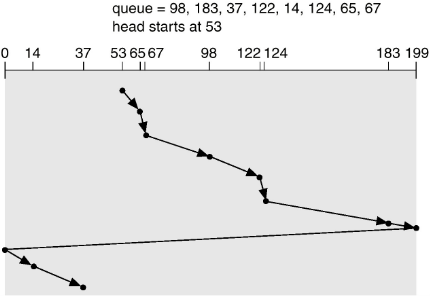
\includegraphics[width=0.5\textwidth]{c-scan.png}
\end{center}
\textbf{SCAN} e \textbf{C-SCAN} evitano la starvation?
No, perché le richieste agli estremi rimangono sempre le 
ultime.

Una soluzione migliore che implementa il meglio degli altri
è una variante dello SCAN, ovvero \textbf{N-step SCAN}, 
la coda delle richieste viene divisa in partizioni grandi 
N, un valore parametrizzato, in questo modo saturate le richieste 
la lista rimane congelata e le servo una dopo l'altra senza 
fermarmi a metà strada, le richieste che arrivano nel mentre 
verranno salvate in una coda diversa. Se il valore di N 
diventasse troppo grande si regredirebbe all'algoritmo 
SCAN, mentre un con valore uguale a 1 si tornerebbe all'
algoritmo FIFO. Con un valore intermedio le cose verrebbero 
gestite decisamente meglio.

La variante più semplicemte e \textbf{FSCAN} (Fast SCAN)
che ha solo due code, si riempie una prima coda e nel 
mentre che viene servita si riempie la seconda, alternandosi 
tra le due.

L'algoritmo \textbf{LIFO} (Last In First Out), in alcuni 
casi avrebbe senso schedulare gli accessi nell'ordine opposto
di arrivo, per dare preferenza a richieste con elevata località.
Pone un alto riscio di starvation, è molto specifico.

Ci sono vari fattori che influenza quale possa essere 
l'algoritmo migliore, nel general purpose il caso medio 
è quello che interessa, mentre in un caso specifico ovviamente 
varia.

\section{Formattazione dei dischi}

Un disco per essere utilizzare deve essere formattato, 
esistono due tipi di formattazione:
\begin{itemize}
    \item basso livello o fisica;
    \item logica.
\end{itemize}
La prima permette di partizionarlo e prepararlo a ricevere 
i dati e iniziare a essere utilizzato. La seconda prepara 
le strutture dati che verranno usate dal SO per gestire 
il disco. Inoltre la formattazione logica va a inserire il 
programma di Bootstrap per caricare i driver dei dispositivi 
e lanciare il SO.
\begin{figure}[h!]
    \centering
    \subfloat[][\textbf{\emph{Disco nudo, preformattazione fisica e logica}}]
    {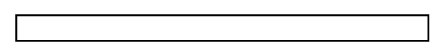
\includegraphics[width=0.5\textwidth]{nuda.png}}\quad
    \subfloat[][\textbf{\emph{Disco post formattazione fisica}}]
    {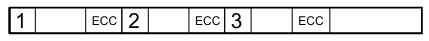
\includegraphics[width=0.5\textwidth]{form_fisica.png}}\\
    \subfloat[][\textbf{\emph{Disco post formattazione logica}}]
    {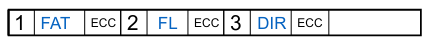
\includegraphics[width=0.5\textwidth]{form_logica.png}}\quad
\end{figure}
La formattazione fisica divide in settori, ogni settore 
avrà uno spazio per i dati e uno per la correzione d'errore,
permettono di ripristinare o identificare un certo numero di 
errori. Se il numero di errori fisici o logici è inferiore 
al numero di errori che possono essere corretti allora si 
potrà continuare a leggere anche in presenza di errori.

La formattazione logica andrà a inserire le strutture 
necessarie per la gestione del file system, capire quali 
blocchi sono liberi e quali sono occupati. 

\section{Gestione dei blocchi difettosi}

Un blocco si può danneggiare per motivi fisici, urti o 
usura, ma anche dei danni software, come un corruzione 
del file system. 

Esistono dei meccanismi di gestione degli errori online, 
un blocco che non funziona lo rimappo in un blocco di scorta.
Il dato non verrà recuperato, però evita di riutilizzare 
il blocco difettoso. I processi continueranno a chiedere 
accessi al blocco difettoso e il SO saprà che dovrà rigirare
tutto al blocco rimappato. Lo svantaggio è che andrà a inficiare 
i meccanismi di scheduling visti sopra, loro saranno convinti 
di andare al blocco con un certo numero, che essendo 
corrotto sarà reindirizzato a un altro blocco che magari si 
trova molto distante causando un aumento del \textbf{Seek Time}.

\section{Gestione dello spazio di swap}

Si tratta di un area in cui vengono salvate pagine e 
frame, non file e cartelle, ma viene gestita alla 
stessa maniera. Le opzioni sono:
\begin{itemize}
    \item definisco l'area non come il file system definendo delle primitive, system call diverse per accedervi;
    \item definisco l'area di memoria virtuale ma la tratto come fosse il file system.
\end{itemize}
Così avremo un sistema meno efficiente perché si avrà a 
che fare con struttre dati inutili per quello che viene 
salvato lì, ma risparmio il dover definire delle 
system call apposite. Viceversa con una partizione 
separata occorerranno le system call ad hoc, ma le 
prestazioni aumenteranno notevolmente.

\chapter{File System}

Consiste di una struttura dati che ci permette di memorizzare 
e organizzare dati e programmi nel modo migliore possibile 
per poterli trovare al momento del bisogno. La struttura 
è simile a quella di un albero, i rami sono le cartelle 
mentre i file sono le foglie.

\section{Interfaccia}

\paragraph{Cos'è un file?} Un file è un'idea astratta 
di uno spazio omogeneo in cui memorizzo dati. Idea 
astratta perché non si sa fisicamente come sia fatto 
o dove si trovi. Un file è uno spazio di indirizzamento 
logico e contiguo. L'unica cosa che lo identifica è 
il nome. Il file può essere di tipi diversi, ha una 
struttura omogenea rispetto all'utilizzo che se ne farà.

\paragraph{Cosa contiene un file?} Oltre ai dati 
che si vogliono memorizzare contiene una parte di attributi,
una sorta di Process Control Block. Gi attributi non sono 
memorizzati dentro al file stesso, ma vengono memorizzate 
all'interno della cartella. Tali attributi sono:
\begin{itemize}
    \item il nome;
    \item il tipo, eseguibile, non eseguibile,...;
    \item la posizione, dove si trova in memoria;
    \item la dimensione;
    \item la protezione, chi può farci e che cosa;
    \item tempo di creazione;
    \item tempo di ultimo accesso;
    \item tempo di ultima modifica;
    \item identità del proprietario.
\end{itemize}
Questi attributi vengono memorizzati in una struttura 
\verb|inode|, che ha bisogno di spazio e viene memorizzata 
all'interno della cartella.

\subsection{Operazioni su file}

\begin{description}
    \item[Creazione]: il SO deve mettere a disposizione delle 
    system call per creare file, che vanno a cercare dello 
    spazio a disposizione per contenere il file.
    \item[Scrittura e lettura]: necessità di sapere la 
    posizione in cui andare a scrivere, analogamente la 
    lettura.
    \item[Cancellazione]: semplicemente rimuove gli 
    attributi dalla directory, ma i dati rimangono in memoria,
    cambia soltanto che non si sa più come raggiungerli.
    I dati spariranno effettivamente con una sovrascrizione
    che non si può sapere quando avverrà effettivamente.
    \item[Troncamento]: lascia il file con gli attributi 
    inalterati, ma azzera la dimensione, ovviamente così 
    il contenuto non viene cancellato.
    \item[Apertura]: impone la ricerca del file all'interno
    della struttura della cartella su disco, la copia in memoria 
    del contenuto e la creazione di due tabelle all'interno 
    delle strutture dati del SO. Una per ogni file aperto 
    e una che lega il file al processo che l'ha aperto.
    Finchè il file è in uso, una sua copia viene 
    caricato in RAM, così da velocizzare lettura e scrittura, 
    la chiusura del file porta al salvataggio permanente 
    su disco.
\end{description}
La rinominazione \textbf{non} è un'operazione su file, 
avviene sulla struttua della cartella, perché cambiare il 
nome di un file consiste nel cambiare la sua posizione, 
il suo pathname.

\subsection{Metodi di accesso}

Un compilatore avrà necessità di accedere al file in modo 
sequenziale, mentre un gestore di base dati dovrà accedervi 
randomicamente

\subsubsection{Sequenziale}

Un processo che vuole accedere a un file in modo sequenziale 
avrà bisogno di operazioni come:
\begin{itemize}
    \item \verb|read next|;
    \item \verb|write next|;
    \item \verb|reset|.
\end{itemize}
In questa modalità di accesso l'operazione di \verb|rewrite| 
non è ammissibile, perché si creerebbe inconsistenza rispetto 
al contenuto precedente, condizione necessaria per un accesso
sequenziale.

\subsubsection{Diretto}

Non interessa partire dall'inizio del file e leggerlo in sequenza, 
quindi ogni elemento del file sarà leggibile e scrivibile 
separatamente dagli altri, il file sarà strutturato a blocchi.
Le operazioni permesse saranno:
\begin{itemize}
    \item \verb|read n|;
    \item \verb|write n|;
    \item \verb|position n|;
    \item \verb|read next|;
    \item \verb|write next|;
    \item \verb|rewrite n|.
\end{itemize}
Non c'è rischio di creare inconsistenza perché ogni file è 
diviso dagli altri(blocchi).

\section{Struttura delle directory}

Il file system è organizzato a volumi o partizioni, è una vista 
logica, quindi indipendente dal numero dei dispositivi fisici.
Esempio: un disco partizionato in due dischi, quindi dal punto 
di vista logico se ne vedranno due. Vale anche la casistica opposta,
due dischi visti dal sistema come un unico disco solo.

All'interno delle partizioni, troviamo una collezione di nodi 
contenenti informazioni sui file. Le directory sono elementi 
che puntano ai file. All'interno della directory verranno memorizzati 
gli attributi dei file visti sopra.

\paragraph{Operazioni su directory}Una volta creata la directory con al suo interno gli \verb|inode|
dei file che vi risiedono si possono compiere le seguenti 
operazioni.
\begin{itemize}
    \item aggiungere file;
    \item cancellare file;
    \item visualizzarne il contenuto;
    \item rinominare un file;
    \item cercare un file;
    \item attraversare il file system.
\end{itemize}

\paragraph{Obiettivi}Gli obiettivi per chi vuole implementare la gestione delle 
directory sono un'elevata efficienza per un accesso rapido al 
file, una nomenclatura che permette agli utenti di 
avere un modo conveniente di dare un nome ai file e
ricordarsi come si chiamano, infine il raggruppamento, ovvero
poter classificare logicamente i file per criterio(tipo, 
protezione, etc...).

\subsection{Directory a un livello}

Unica per tutti gli utenti, la nomenclatura era un problema 
perché ogni file doveva avere un nome differente rispetto 
agli altri, considerando che la lunghezza massima dei file 
al tempo era di 8 caratteri.
\begin{center}
    \foto{mono_dir.png}
\end{center}

\subsection{Directory a due livelli}

Una prima evoluzione è stata la separazione delle cartelle 
a livello utente, è nato un primo concetto di cartella \verb|home|
per ogni utente e al suo interno ogni utente metteva i loro file.
La problematica sulla nomenclatura si spostava, ora non era più condivisa tra 
tutti gli utenti, ma era per il singolo che all'interno della sua
cartella non poteva crearne altre e di conseguenza era limitato 
con la rinomina dei file. Nasce anche il problema di decidere 
dove posizionare i programmi di sistema, se replicarli 
all'interno di ogni singola cartella o no, da cui nasce a 
sua volta il concetto di variabile di ambiente, che permettono di 
specificare cose come il PATH. Sulle macchine Linux 
tale variabile d'ambiente contiene cartelle e sottocartelle 
con programmi eseguibili che permettono di essere lanciati da terminale.
\begin{center}
    \foto{bi_dir.png}
\end{center}

\subsection{Directory ad albero}

Permettono una ricerca efficiente, attraversando l'albero 
aggiungendo la possibilità di raggruppare sotto cartelle,
nasce l'idea della directory corrente o directory '.', 
di comandi \verb|cd| o \verb|pwd|. Nasce il concetto di percorso 
assoluto e relativo ovvero relativo alla posizione attuale. Uno 
'/' all'inizio del percorso indicherà un percorso assoluto, ovvero 
dalla radice, mentre ometterlo indicherà un percorso relativo 
ovvero partendo dalla locazione attuale in cui ci si trova.
\begin{center}
    \foto{dir_albero.png}
\end{center}

\subsection{Directory a grafo aciclico}

Ci saranno dei rami che si ricongiungono, facilitando la condivisione 
tra utenti. Da questo nasce il concetto di link, simbolici 
e hard link. 
\begin{description}
    \item[Link simbolico:] un altro file con all'interno il pathname del file a cui si collega;
    \item[Hard link:] il file è uno solo, al quale fa riferimo un \verb|inode1| e quello del link \verb|inode2|, un unico file con due strutture di attributi diversi.  
\end{description}
Cancellando un \verb|inode| a un hard link il file rimarrà, fintanto che avrà 
un collegamento con un altro \verb|inode|. Se si cancella un 
link simbolico, il file originale rimarrà, ma se si cancellasse 
il file a cui il link simbolico punta, avremo un errore 
tentando di aprirlo siccome non punterà più a nulla.
Una modifica eseguita a un file tramite hard link sarà 
visibile pure tramite l'altro link.
\begin{center}
    \foto{dir_grafo.png}
\end{center}

\subsection{Directory a grafo generico}

Con questa struttura ci sono possono essere dei cicli, 
ciò potrà causare dei problemi eventualmente con la 
ricerca. In tal caso bisognerà usare degl algoritmi di controllo 
dei cicli per verificare se nel link creato sia nato un 
ciclo o meno.
\begin{center}
    \foto{dir_gen.png}
\end{center}

\subsection{Mount di file system}

Meccanismo che permette di collegare un punto del 
file system corrente a un altro file system, in modo 
da poterlo raggiungere e attraversare come se facesse 
parte del nostro file system, esempio: quando si collega 
una chiavetta USB.

\section{Protezione}

Potendo creare file system grandi a piacere con cartelle 
a grafo, occorre pensare anche ai livelli di protezione 
per impedire che un utente faccia cose indesiderate sul file 
system. Esistono varie possibilità per permettere al proprietario 
del file di fare qualsiasi cosa. Si parte decidendo che tipo di 
operazioni controllare, dando dei permessi:
\begin{itemize}
    \item lettura;
    \item scrittura;
    \item esecuzione;
    \item append;
    \item cancellazione;
    \item ...
\end{itemize}
Un primo livello di protezione è un inserimento in ogni 
directory di un elenco di chi può fare cosa. Molto 
complicato da gestire ed estremamente lungo. Un meccanismo 
più efficiente e meno fine è il raggruppamento in 3 classi
usato dai sistemi Unix. Ogni file apparterrà all'utente che
l'ha creato, quell'utente appartiene a un gruppo di utenti 
che condividono un certo insieme di privilegi. Gli 
utenti sono divisi in 3 categorie:
\begin{itemize}
    \item proprietario;
    \item il gruppo di utenti a cui appartiene il proprietario;
    \item tutti gli altri.
\end{itemize}
Ogni utente può appartenere a più gruppi contemporaneamente.
I permessi per ogni classe verranno identificati tramite 
i caratteri \verb|r|, \verb|w| e \verb|x|. Per un cartella 
il permesso di execute \verb|x|, corrisponde alla possibilità 
di poterla attraversare tramite il comando \verb|cd|.

\section{Implementazione del file system}

Il file system è strutturato in un insieme di livelli che 
implementano una serie di funzionalità sfruttando quello che 
viene offerto dal livello inferiore per offrirne al livello superiore (strutturazione modulare).
Nella parte più bassa ci sono i dispositivi di memorizzazione 
di massa, controllati dai device driver, ovvero software 
creati per permettere al SO di riconoscere le funzionalità 
delle periferiche. Esistono devide driver generici, ovvero 
compatibili con la tipologia di device driver e permettono 
di avere un meccanismo plug 'n play.

I \textbf{device driver} al loro interno implementano il primo livello 
di gestione: I/O Control, quella parte che gestisce anche 
l'aspetto relativo alla gestione dell'interrupt, garantisce 
l'interazione tra periferica e sistema e implementa la 
gestione fisica della scrittura dei blocchi e lettura da 
periferica verso la memoria. 

A livello di \textbf{I/O Control} c'è il disk scheduling 
e gestione di lettura/scrittura fisica dei blocchi, queste 
azione vengono effettuate a fronte di comandi implementati 
a livello di \textbf{basic file system}, comandi indipendenti dal device 
driver o periferica specifica, astraggono l'idea di scrivere/leggere 
blocchi di dati. Al suo interno si troverano primitive che 
ci permetteranno di scrivere/leggere un blocco. Questi comandi 
arrivano dal \textbf{file-organization module}, dove non si 
parla più di blocchi, ma l'entità minima è il file. In questa zona 
si troveranno operazioni che permettono di tradurre dove si trova 
fisicamente un blocco logico nello spazio fisico.

Il livello superiore sarà il \textbf{logical file system} 
ovvero l'interfaccia tra programmi e utente.

Per gestire l'implementazione di un file system, sarà necessario 
creare delle strutture dati, alcune risiederanno in memoria per 
motivi di efficienza e altre su disco per motivi di non 
volatilità e successivamente caricate in memoria per migliorare 
l'accesso e renderlo più rapido.

\subsection{Strutture su disco}

All'interno del disco si troveranno aree dedicate a:
\begin{itemize}
    \item gestire il blocco di boot, ovvero gestire le info 
    di avvio del sistema, quando si avvia la macchina, questa 
    andrà a verificare una spefica area su disco, l'area di boot,
    fondamentale per l'avvio;
    \item blocco di controllo delle partizioni, descrive come i 
    vari dischi sono stati distribuiti dal punto di vista logico
    come visto più su;
    \item strutture delle directory
    \item descrittori dei file (inode), contengono gli attributi 
    tra cui quelli che indicano dove si trovano i blocchi dei file 
    fisicamente su disco.
\end{itemize}

\subsection{Strutture in memoria}

\begin{itemize}
    \item tabella delle partizioni, contengono informazioni 
    sulle partizioni montate e che sono visibili all'utente;
    \item struttura delle directory, presente anche in memoria 
    per una gestione più rapida;
    \item tabella globale dei file aperti, contiene la copia 
    del descrittore del file dei file aperti;
    \item tabella dei file aperti per ogni processo, contiene in particolare 
    informazioni riguardo la copia file aperto-processo; 
\end{itemize}

\subsection{Allocazione dello spazio su disco}

L'obiettivo è di alloccare spazio su disco per file e cartelle, 
cercando di massimizzare l'uso del disco senza sprecare spazio 
(ridurre le strutture di controllo e di gestione come le cartelle)
e minimizzare i tempi di accesso su disco. Le possibili
alternative sono:
\begin{itemize}
    \item allocazione contigua;
    \item allocazione a lista concatenata (linked);
    \item allocazione indicizzata;
\end{itemize}

\subsubsection{Allocazione contigua}

Simile a quella in memoria.
\begin{itemize}
    \item \textbf{Vantaggi}:
    \begin{itemize}
        \item semplifica la struttura della directory, 
        la directory dovrà solo memorizzare il blocco 
        di partenza del file e la sua dimensione, con solo 
        queste due info potrà accedere al file;
        \item accesso semplice, se si è al blocco B l'accesso 
        al blocco successivo sarà semplicemente al blocco B+1
        inoltre permette l'accesso sia sequenziale che casuale, 
        per andare al blocco i-esimo basterà fare B+i;
    \end{itemize}
    \item \textbf{Svantaggi}:
    \begin{itemize}
        \item necessità di avere meccanismi di ricerca di
        uno spazio sufficientemente grande, portando a creare
        frammentazione esterna (effetto groviera);
        \item cosa succede se il file cresce? lo si limita 
        per impedire che cresca ulteriormente o si trova una 
        nuova zona più spaziosa con lo spostamento di tutto 
        il file da un'area a un'altra;
    \end{itemize}
\end{itemize}

\subsubsection{Allocazione a lista (linked list)}

Si taglia a blocchi di equa dimensione il file, ogni 
file sarà una lista di blocchi che possono essere 
locati ovunque. La directory conterrà per ogni file il 
puntatore per il primo blocco il quale al suo interno 
conterrà il puntatore al blocco successivo. La directory
avrà anche il puntatore all'ultimo blocco, nel caso di 
errori come blocchi difettosi o errori software che portano 
a rovinare un blocco della lista e di conseguenza impedire 
la lettura dei blocchi successivi, con il puntatore 
all'ultimo blocco si potrà provare a ricostruire il file.
Questo è possibile perché ogni blocco punta a quello successivo 
e a quello precedente, ovviamente nel caso in cui un intero 
blocco fosse completamente compromesso, il file sarebbe 
spezzato a metà e irrecuperabile. 

Esempio di indirizzamento:
\begin{lstlisting}[language=C]
    X = indirizzo logico
    N = dimensione del blocco
    /*per capire a quale blocco leggere*/
    X / (N - 1)
    /*per capire quanto leggere di quel blocco*/
    X % (N - 1)
\end{lstlisting}
N.B.: il -1 è dovuto alla presenza del puntatore che ovviamente 
non deve essere considerato per leggere o scrivere su un blocco.
\begin{itemize}
    \item \textbf{Vantaggi}:
    \begin{itemize}
        \item creare un nuovo file è semplice, si trova un 
        blocco libero e ci si scrive al suo interno, nel caso 
        di necessità di altri blocchi se ne trova un altro 
        libero (recuperandolo dalla \textbf{free list}, la 
        lista dei blocchi liberi in memoria), lo si 
        concatena e si prosegue ci sarà uno spreco minimo 
        perché occorrerrà solo mettere due puntatori per blocco
        evitando la frammentazione esterna;
    \end{itemize}
    \item \textbf{Svantaggi}:
    \begin{itemize}
        \item l'accesso casuale non è facile da fare, se 
        si vuole leggere a metà di una lista linkata 
        sarà sempre necessario scorrerla completamente e 
        se i blocchi si trovano sparpagliati per il disco 
        la testina dovrà continuamente muoversi portando 
        ad aumentare il tempo di lettura;
        \item affidabilità, spiegato sopra, se un blocco dovesse 
        corrompersi completamente il file rimarrebbe troncato 
        e irrecuperabile;
    \end{itemize}
\end{itemize}
\paragraph{Esempio - FAT (File Allocation Table)} usata nei 
sistemi MS-DOS, la cartella aveva il nome del file e il blocco di partenza, 
questo blocco non puntava alla zona del disco in cui si trovava, 
ma a una tabella allocata contiguamente su disco e compatta, con 
all'interno solamente l'insieme di puntatori a ogni blocco.

\paragraph{Variante con allocazione contigua} si crea una 
lista di aree contigue invece di una lista di blocchi, 
permette di aumentare l'efficienza, siccome leggere un'area 
contigua è più veloce rispetto a leggere blocchi. Un'area 
contigua si definirà \textbf{extent} lunga quanto possibile, 
alla creazione di un file si prenderà la prima area contigua disponibile,
il primo \textbf{extent} e si memorizzerà ciò che interessa.
Se il file dovesse crescere, si cercheranno dei blocchi 
liberi contigui, se si trovano si aumenterà l'\textbf{extent} in 
alternativa si andrà alla ricerca di un'altra area libera 
e si concateneranno gli \textbf{extent} senza la necessità 
fare allocazione dinamica e causare frammentazione.

\subsubsection{Allocazione indicizzata}

Ogni directory contiene la \textbf{index table} (simile 
alla tabella delle pagine) che contiene le 
informazioni riguardo i blocchi costituenti del file
\begin{center}
    \foto{index_table.png}
\end{center}
I -1 sono ulteriori puntatori a blocchi che potranno essere 
utilizzati per accrescere il file.

L'allocazione indicizzata ha un accesso sequenziale e casuale efficiente, 
posso accedere a qualunque posizione del file nello stesso tempo, 
seguendo gli indici della tabella. Ha un accesso dinamico
senza necessità di frammentazione esterna, posso prendere 
qualunque blocco libero e farlo puntare dalla tabella dei 
blocchi, il costo è maggiore rispetto all'allocazione 
a lista, perché qui servirà un blocco per ogni file.

Esempio di indirizzamento:
\begin{lstlisting}[language=C]
    X = indirizzo logico
    N = dimensione del blocco
    /* ottengo la riga della tabella dove
    andare a leggere */
    X / N = offset della index table
    X % N = offset all'interno del blocco dati
\end{lstlisting}

La dimensione del blocco limiterà la dimensione del file.
Per superare queste dimensione si applicano:
\begin{itemize}
    \item indici multilivello;
    \item schema concatenato;
    \item schema combinato.
\end{itemize}

\paragraph{Indici multilivello} simile alle tabelle delle 
pagine a più livello, ogni riga di un indice base di primo 
livello punterà a una tabella di indici di secondo livello
che potrà a sua volta puntare ad altre tabelle di indici oppure 
direttamente ai blocchi con i dati desiderati.

Esempio:
\begin{itemize}
    \item Tabella più esterna contiene puntatori
    alle index table
    \begin{itemize}
        \item X = indirizzo logico  
        \item N = dimensione del blocco(in parole)
        \begin{itemize}
            \item X / (N * N) = blocco della index table 1° livello
            \item X \% (N * N) = R
        \end{itemize}
        \item R usato come segue
        \begin{itemize}
            \item R / N = offset nel blocco della index table 
            di 2° livello
            \item R \% N = offset nel blocco dati
        \end{itemize}
    \end{itemize}
    \item Es.: blocchi da 4KB consentono 1K indici da 4B 
        -> due livelli di indici consentono file da 4GB
\end{itemize}

\paragraph{Schema concatenato} si prende un primo blocco 
indice e si usano tutti i puntatori per indirizzare il 
file, l'ultimo se serve ancora spazio punterà a un altro 
blocco indice, in cui tutti i puntatori verranno usati 
alla stessa maniera. La lista di blocchi indice sarà lunga 
quanto sarà necessario per indirizzare il file.

L'indirizzamento sarà:
\begin{itemize}
    \item X = indirizzo logico
    \item N = dimensione del blocco (in parole)
    \begin{itemize}
        \item X / (N(N - 1)) = numero del blocco indice 
        all'interno della lista dei blocchi indice
        \item X \% (N(N - 1)) = R 
    \end{itemize}
    \item R usato come segue
    \begin{itemize}
        \item R / N = offset nel blocco indice
        \item R \% N = offset nel blocco dati
    \end{itemize}
\end{itemize}

Esempio:
\begin{itemize}
    \item N = 1KB = 256 parole
    \begin{itemize}
        \item 4 B per parola
    \end{itemize}
    \item Max file = 256 blocchi da 1KB = 256KB
    \begin{itemize}
        \item X = 12200
        \begin{itemize}
            \item X / N = 12200 / 256 = 47(blocco 47)
            \item X \% N = 168(parola 168 in blocco 47)
        \end{itemize}
        \item X = 644000 non basta un primo livello
        \begin{itemize}
            \item X / (N(N - 1)) = 9(blocco lista)
            \item X \% (N(N - 1)) = R = 56480
            \item R / N = 220(offset nel blocco indice)
            \item R \% N = 160(offset nel blocco dati)
        \end{itemize}
    \end{itemize}
\end{itemize}

\section{Implementazione delle directory}

Viene utilizzato lo stesso meccanismo usato per memorizzare 
i file, da ricordare che le directory non contengono dati, 
ma avranno degli inode. Nelle directory principalmente 
si eseguono delle ricerche dei file, per ottimizzare 
le ricerche al loro interno ci sono delle tabelle hash

\section{Gestione dello spazio libero}

Struttura dati necessaria per tenere traccia dei 
blocchi che si possono usare per creare un nuovo file 
o per estenderne uno esistente. Quando un file viene 
eliminato la struttura verrà aggiornata con i blocchi 
disponibili. Esistono 4 forme/modalità di utilizzo differenti:
\begin{itemize}
    \item vettore di bit;
    \item lista concatenata;
    \item raggruppamento;
    \item conteggio.
\end{itemize}

\subsection{Vettore di bit} 

Consiste di un vettore composto da tanti elementi quanti 
sono i blocchi del sistema di memorizzazione di massa, 
all'interno ci sarà un 1 (blocco disponibile) o uno 0 
(blocco occupato). Quando si avrà bisogno di cercare un
blocco per un nuovo file si scorrerà il vettore alla 
ricerca di un elemento con all'interno un 1, sapendo 
eventualmente quanti blocchi servono per tempo si potranno
cercare aree con quel numero di blocchi liberi contigui 
per velocizzare i tempi di accesso.

Un contro di questo meccanismo è che richiede spazio extra 
per tenere traccia di questo vettore, che occuperà spazio 
sia su disco che in memoria. 

\subsection{Lista concatenata}

Spreca poco spazio, perché non è necessario avere 
un vettore di bit, è solamente necessario avere un 
puntatore a una lista, che punterà al primo, a sua volta 
al secondo, etc. 

Lo svantaggio è che non si può tenere spazio contiguo 
facilmente. 

\subsection{Raggruppamento}

Una possibile miglioria è l'uso di una lista con un 
raggruppamento, il primo blocco libero non punta 
al successivo, ma a una lista di blocchi liberi, una sorta 
di lista indicizzata, rendendo facile recuperare gruppi 
di blocchi liberi.

\subsection{Conteggio}

All'interno di un blocco disponibile si andrà a scrivere 
quanti blocchi contigui sono disponibili dopo di esso, 
il puntatore in questo caso punterà al blocco libero
successivo non contiguo.

\section{Efficienza e prestazioni}

Il disco fisso è il collo di bottiglia rispetto al resto, 
esiste la possibilità di migliorare le prestazioni.
\begin{itemize}
    \item ram disk;
    \item buffer cache.
\end{itemize}
Il disco ha un controllore che contiene un buffer per una 
traccia, una alla volta viene trasferita tramite il controllore 
alla memoria principale. In memoria si potrà creare un'ulteriore 
area di cache, in cui memorizzare le tracce a cui si è fatto 
accesso più recentemente. I programmi così se dovranno 
riutilizzare tracce già visitate, le troveranno disponibili
all'interno di questa cache. 

Un'altra possibilità è di creare un disco virtuale, localizzato 
in RAM, per velocizzare l'accesso.

\subsection{Dischi virtuali}

Una parte della RAM verrà utilizzata per memorizzare file,
dal punto di vista dei processi, le stesse primitive usate 
per leggere su disco fisso andranno bene pure sul disco
virtuale. \textbf{N.B.}: non è una cache, viene gestita 
dall'utente.

Questa funzione ovviamente va bene per i file temporanei.

\subsection{Buffer cache}

In memoria RAM, ma usata come cache e controllata dal 
SO, memorizzerà i blocchi visitati più frequentemente 
in modo di evitare accessi al disco, funziona grazie al 
principio della località temporale.

\subsection{File system log structured}

Quando viene richiesto di scrivere su un file, con questo 
file system la scrittura non avverrà sui blocchi 
fisici associati ai file, ma su dei blocchi di un file di 
log in cui il sistema scrive tutto ciò che avviene. 
In questo modo si evita lo spreco di tempo della testina 
sul disco, scrivendo tutto sequenzialmente su questo blocco 
di log. Infine quando il disco sarà inutilizzato, avverrà 
la scrittura effettiva sui blocchi associati. Questa 
funzione è resistente ai crash, siccome il file rimarrà
salvato.  





    
    



















\end{document}